
\documentclass[12pt]{report}

% ---------------- Packages ----------------
\usepackage[utf8]{inputenc}
\usepackage[a4paper, left=1.25in, right=1in, top=1in, bottom=1in]{geometry}
\usepackage{setspace}
\usepackage[titletoc]{appendix}
\usepackage{graphicx}
\usepackage{float}
\usepackage{multirow}
\usepackage{booktabs}
\usepackage{array}
\usepackage{longtable}
\usepackage{algorithm}
\usepackage{algpseudocode}
\usepackage{listings}
\usepackage{colortbl}
\usepackage{xcolor}
\usepackage{caption}
\usepackage{subcaption}
\usepackage{cite}
\usepackage{hyperref}
\usepackage{lmodern}
\usepackage{sectsty}
\usepackage{ulem}
\usepackage{nomencl}
\usepackage{ragged2e}

% ---------------- Graphics Path ----------------
\graphicspath{{images/}}

% ---------------- Hyperlink Setup ----------------
\hypersetup{
    colorlinks,
    citecolor=red,
    filecolor=black,
    linkcolor=black,
    urlcolor=blue
}

% ---------------- Compact Formatting ----------------
\setstretch{1.25}
\setlength{\parindent}{0pt}
\setlength{\parskip}{0.45em}
\raggedbottom

% Reduce extra space around figures/tables
\setlength{\textfloatsep}{8pt plus 2pt minus 2pt}
\setlength{\floatsep}{8pt plus 2pt minus 2pt}
\setlength{\intextsep}{8pt plus 2pt minus 2pt}
\setlength{\abovecaptionskip}{4pt}
\setlength{\belowcaptionskip}{2pt}
\captionsetup{font=small, skip=4pt}

% ---------------- Chapter / Section Font Size ----------------
\chapterfont{\fontsize{20pt}{22pt}\selectfont\bfseries}
\sectionfont{\fontsize{14pt}{16pt}\selectfont\bfseries}
\subsectionfont{\fontsize{12.5pt}{14pt}\selectfont\bfseries}

\makeatletter
\renewcommand\@seccntformat[1]{\csname the#1\endcsname\enspace}
\makeatother

% ---------------- Table Column Types ----------------
\newcolumntype{Y}{>{\centering\arraybackslash}m{4.4cm}}
\newcolumntype{X}{>{\centering\arraybackslash}m{7cm}}
\newcolumntype{P}{>{\centering\arraybackslash}m{2.5cm}}
\newcolumntype{L}{>{\raggedright\arraybackslash}m{8cm}}
\newcolumntype{M}{>{\raggedright\arraybackslash}m{3.7cm}}
\newcolumntype{Z}{>{\justify\arraybackslash}m{15cm}}

% ---------------- Other Commands ----------------
\newcommand{\etal}{\textit{et al. }}
\newcommand{\myrowcolour}{\rowcolor[gray]{0.925}}
\renewcommand\bibname{References}
\makenomenclature

% ---------------- Document Starts ----------------
\begin{document}

% Roman page numbering for preliminary pages
\renewcommand{\thepage}{\roman{page}}
\setcounter{page}{1}

\begin{titlepage}
    \begin{center}
        
        % This template is created and modified by Rashik Rahman(17201012@uap-bd.edu). Feel free to contact me if you have any quarries or problems regarding this template. 
        
        %%Author Social links
        %%Git : https://github.com/RashikRahman
        %%Google scholar : https://scholar.google.com/citations?user=20fAehwAAAAJ&hl=en
        %%Linkedin : https://www.linkedin.com/in/rashik-rahman-5a327a1a6/
        %%Facebook : https://www.facebook.com/rashikrahman.pritom.7/
        
        
        \LARGE
        \textbf{Automated Car Parking System}
         
        \par 
        \large
        
Submitted as a Final Lab Project Report for the Course Robotics Lab\\
Department of Computer Science and Engineering\\
University of Asia Pacific\\


        \vspace{1cm}
        
        by
        \Large
        \par
        \textbf{Md Shahid Al Mamim}\\ID: 22201181\\
        \vspace{0.2cm}
        \textbf{Md Mizanur Rahman}\\ID: 22201189\\
        \vspace{0.2cm}
        \textbf{Lamia Akter Jesmin}\\ID: 22201190\\
        
        \vspace{1.5cm}
        Supervised by:\\
        \Large
        \textbf{Dr. Nazmun Nahid}\\Assistant Professor\\
        \vspace{0.2cm}
        
        % \vfill

         \vspace{1cm}
        
              
     
          
            
        
\includegraphics[width=0.2\textwidth]{images/logo.png}\\
        \vspace{0.2cm}   
        \large
        \textbf{Department of Computer Science \& Engineering}\\
        \large
        \textbf{University of Asia Pacific}\\
           \vfill
        
        \vspace{0.5cm}
        \large
        \textbf{June 2026}\\
        \vspace{0.8cm}

    \end{center}
\end{titlepage}


\newpage
\begin{center}

    \vspace*{0.1cm}
    \large
    \textbf{Certificate of Approval}\\
    \vspace{0.5cm}

\end{center}

\noindent
{\large This is to certify that the project report entitled \textbf{``Automated Car Parking System''} has been prepared by \textbf{Md Shahid Al Mamim}, \textbf{Md Mizanur Rahman}, and \textbf{Lamia Akter Jesmin} as a final lab project report for the course \textbf{Robotics Lab} under the Department of Computer Science and Engineering, University of Asia Pacific. The report is accepted as a satisfactory submission for the course requirement.}

\vspace{2cm}

\begin{flushright}
Course Instructor
\end{flushright}

\vspace{-2.3cm}

................................................................................\\
\textbf{Dr. Nazmun Nahid}\\
Assistant Professor\\
Department of Computer Science and Engineering\\
University of Asia Pacific (UAP)

\vspace{2.5cm}

\begin{flushright}
Head of the Department
\end{flushright}

\vspace{-2.3cm}

................................................................................\\
\textbf{Prof. Dr. Shah Murtaza Rashid Al Masud}\\
Professor and Head\\
Department of Computer Science and Engineering\\
University of Asia Pacific (UAP)



\newpage
\thispagestyle{plain}
\begin{center}

    \vspace*{0.1cm}
    \Large
    \textbf{Acknowledgements}\\
    \vspace{0.5cm}

\end{center}

First of all, we would like to express our sincere gratitude to Almighty Allah for giving us the strength, patience, and ability to complete this project successfully.

We would like to express our deepest gratitude to our respected course instructor, \textbf{Dr. Nazmun Nahid}, Assistant Professor, Department of Computer Science and Engineering, University of Asia Pacific, for her valuable guidance, support, and encouragement throughout the development of this project. Her instructions and suggestions helped us understand the project requirements and complete the work in a proper and organized way.

We are also thankful to the Department of Computer Science and Engineering, University of Asia Pacific, for providing us with the opportunity to work on this robotics lab project. The knowledge gained from the course helped us apply concepts of robotics, embedded systems, sensors, actuators, and IoT communication in a practical project.

We would like to thank our group members for their cooperation, teamwork, and dedication during the planning, hardware setup, coding, testing, and report writing stages of the project. The successful completion of the \textbf{Automated Car Parking System} was possible because of the combined effort of all team members.

Finally, we are grateful to our families and friends for their continuous support, motivation, and encouragement throughout the project work.



\newpage
\begin{center}

    \vspace*{0.05cm}
    \Large
    \textbf{Abstract}\\
    \vspace{0.5cm}

\end{center}

Parking management is a major challenge in urban areas because manual systems often cause delay, confusion, and inefficient use of parking spaces. This project presents an \textbf{Automated Car Parking System} that integrates robotics and IoT technologies to automate vehicle entry, exit, and parking slot monitoring. The system uses Arduino UNO as the main controller, IR sensors for vehicle detection, RFID for authorized access, a 16x2 I2C LCD for displaying available slots, an ESP-01S Wi-Fi module for online data transmission, and a servo motor-controlled two-link robotic arm as the gate mechanism. When a vehicle is detected at the entrance, the system checks slot availability and requests RFID authentication. If the card is valid, the robotic arm gate opens, the slot count is updated, and the entry record is sent to the online server. During vehicle exit, the system detects the vehicle, opens the gate, updates the slot count, and stores the exit record. The prototype was tested under different entry and exit conditions, and the results showed successful vehicle detection, RFID verification, robotic gate operation, LCD update, and IoT data transmission. The proposed system reduces manual effort, improves parking efficiency, and demonstrates a practical application of robotics and IoT in smart parking management.



\tableofcontents

\addcontentsline{toc}{chapter}{List of Figures}
\listoffigures

\addcontentsline{toc}{chapter}{List of Tables}
\listoftables

% Arabic page numbering for main chapters
\clearpage
\setcounter{page}{1}
\setcounter{chapter}{0}
\renewcommand{\thepage}{\arabic{page}}
\setlength{\parskip}{0.45em}

% ---------------- Chapters ----------------

\chapter{Introduction}
\label{cha:introduction}

In recent years, rapid urbanization and the increasing number of vehicles have made parking management a major challenge in residential, commercial, institutional, and public areas. Traditional parking systems usually depend on manual gate control, manual slot checking, and manual record keeping. This process is time-consuming, less accurate, and inefficient when the number of vehicles is high.

Automation, robotics, embedded systems, and Internet of Things (IoT) technologies can improve parking management by detecting vehicles, verifying access, controlling gates, updating available slots, and storing parking data automatically. In this project, an \textbf{Automated Car Parking System} is designed using Arduino UNO, IR sensors, RFID, LCD display, ESP-01S Wi-Fi communication, and a servo motor-controlled two-link robotic arm gate mechanism.

The system detects a vehicle at the entrance using an IR sensor and checks parking slot availability. If a slot is available, the user scans an RFID card for authentication. After successful verification, the Arduino controls the servo motor to move the two-link robotic arm gate. The available slot count is updated on the LCD and the entry record is sent to an online server. During exit, the system detects the vehicle, opens the robotic arm gate, increases the available slot count, and stores the exit record. Thus, the proposed system combines robotic gate control and IoT-based monitoring to create a low-cost smart parking prototype.

\section{Background and Motivation}

Parking space management has become difficult in busy places such as shopping malls, offices, universities, hospitals, and residential buildings. Drivers often waste time searching for available parking spaces, which increases congestion near parking areas. Manual systems may also create errors in slot counting and vehicle entry-exit records.

The motivation of this project is to develop a simple, low-cost, and automated parking system suitable for academic prototype implementation. The system uses IR sensors for vehicle detection, RFID for authorized access, an LCD for real-time slot display, ESP-01S for online data transmission, and a two-link robotic arm as the gate mechanism. The robotic arm adds a robotics-based control feature and demonstrates practical use of actuator movement in parking automation.

\section{Problem Statement}

Traditional parking systems have several limitations. Manual gate operation can cause delays during vehicle entry and exit. Manual slot counting can be inaccurate, and drivers may not know whether parking space is available before reaching the gate. Manual record keeping is also difficult to maintain for a long time.

Security is another concern in controlled parking areas. Without authentication, unauthorized vehicles may enter the parking area. Therefore, an automated system is needed that can detect vehicles, verify authorized users, control the gate, update slot availability, and store parking data using IoT communication.

\section{Objectives of the Project}

The main objective of this project is to design and implement an Automated Car Parking System that can control vehicle entry and exit using sensors, RFID, microcontroller-based control, IoT communication, and a two-link robotic arm gate.

The specific objectives are:

\begin{enumerate}
    \item To design a prototype automated parking system using Arduino UNO.
    \item To detect vehicles at entry and exit points using IR sensors.
    \item To use RFID for authorized vehicle entry.
    \item To control a servo motor-based two-link robotic arm gate.
    \item To display available parking slots on a 16x2 I2C LCD.
    \item To update parking slot count automatically after entry and exit.
    \item To send entry and exit records to an online server using ESP-01S.
    \item To demonstrate the integration of robotics and IoT in parking automation.
\end{enumerate}

\section{Research Questions}

The project is guided by the following research questions:

\begin{enumerate}
    \item How can an Arduino-based system automate vehicle entry and exit?
    \item How effectively can IR sensors detect vehicle presence?
    \item How can RFID be used for authorized parking access?
    \item Can a servo-controlled two-link robotic arm operate as a reliable gate?
    \item How can parking slot information be updated and stored automatically?
\end{enumerate}

\section{Scope of the Work}

This project focuses on a prototype-level Automated Car Parking System. The system uses Arduino UNO, IR sensors, RFID module, ESP-01S Wi-Fi module, LCD display, and a servo motor-controlled two-link robotic arm. The main functions include vehicle detection, RFID authentication, robotic gate control, parking slot counting, LCD-based status display, and IoT-based data transmission.

The scope is limited to a small-scale lab prototype. It does not include automatic number plate recognition, camera-based detection, payment system, mobile reservation, GPS guidance, or large-scale commercial deployment. However, these features can be added in future versions.

\section{Expected Outcomes}

The expected outcome is a functional prototype that can detect vehicles, verify RFID cards, operate the two-link robotic arm gate, update slot availability, display parking status, and send parking records online. The system is expected to reduce manual effort, improve parking efficiency, and demonstrate the practical application of robotics and IoT in smart parking management.

\section{Impacts of the Project}

The proposed system can improve parking management by reducing manual gate operation and manual slot counting. It can save time for drivers, reduce congestion near parking gates, and support more organized parking control. Since the system stores parking data online, data privacy and secure communication should be considered in real deployment.

\subsection{Impact on Societal and Cultural Issues}

The system can support society by making parking more efficient and reducing waiting time. It also encourages the use of automation and IoT-based solutions in daily life, supporting smart city development and technology awareness.

\subsection{Impact on Health, Safety, and Legal Issues}

The automated gate operation can reduce human error and improve safety during vehicle entry and exit. The system has no direct health impact, but it can reduce driver stress by making parking faster. From a legal perspective, RFID and entry-exit data should be protected from unauthorized access.

\subsection{Impact on Environment and Sustainability Issues}

Efficient parking management can reduce unnecessary vehicle movement and waiting time, which may help lower fuel consumption and emissions. The system also uses low-cost and low-power electronic components suitable for sustainable prototype development.

\section{Report Organization}

The report is organized as follows:

\textbf{Chapter 1: Introduction}\\
This chapter presents the background, motivation, problem statement, objectives, scope, expected outcomes, impacts, and report organization.

\textbf{Chapter 2: Related Works}\\
This chapter reviews existing smart parking systems, IoT-based parking management, RFID access control, and automated gate systems.

\textbf{Chapter 3: System Analysis and Design}\\
This chapter describes requirements, system architecture, hardware setup, circuit connection, and robotic arm gate structure.

\textbf{Chapter 4: Methodology and Implementation}\\
This chapter explains the development method, tools, data handling, algorithm, flowchart, and module implementation.

\textbf{Chapter 5: Results and Evaluation}\\
This chapter presents testing setup, performance metrics, result analysis, discussion, and limitations.

\textbf{Chapter 6: Project Planning and Budget}\\
This chapter includes the project timeline, cost estimation, and resource planning.

\textbf{Chapter 7: Standards and Design Constraints}\\
This chapter discusses standards, design constraints, CEP, CEA, and knowledge profile mapping.

\textbf{Chapter 8: Conclusion and Future Work}\\
This chapter summarizes the project achievements, limitations, and future improvement possibilities.



\chapter{Related Works}
\label{cha:LiteratureReviewU}

This chapter presents the background concepts, related works, and existing systems associated with the proposed \textbf{Automated Car Parking System}. It briefly explains the main technologies used in the project and identifies the limitations of existing parking solutions.

\section{Preliminaries}

The proposed system combines embedded systems, sensors, RFID authentication, robotic actuation, LCD display, and IoT-based data communication. These components work together to detect vehicles, verify users, control the gate, update parking slots, and store parking records online.

\subsection{Internet of Things}

The Internet of Things (IoT) connects physical devices to the internet for data exchange and remote monitoring \cite{b7}. In this project, IoT is used to send vehicle entry and exit records to an online server or database through the ESP-01S Wi-Fi module.

\subsection{Embedded System and Arduino UNO}

An embedded system is designed to perform a specific task using hardware and software. The Arduino UNO works as the main controller of this project. It receives input from IR sensors and the RFID module, processes the logic, controls the servo motor, updates the LCD, and communicates with the Wi-Fi module \cite{b9}.

\subsection{IR Sensor}

IR sensors are used to detect vehicle presence at the entry and exit points. When a vehicle is detected, the sensor sends a digital signal to the Arduino, which starts the entry or exit process.

\subsection{RFID Technology}

RFID is used for contactless identification. In this project, the RFID reader scans a card UID and compares it with authorized IDs. If the card is valid, the system allows the vehicle to enter; otherwise, access is denied \cite{b11}.

\subsection{Servo Motor and Two-Link Robotic Arm}

A servo motor provides controlled angular movement and is commonly used in robotics \cite{b10}. In this project, the servo motor controls a two-link robotic arm that works as the automatic gate mechanism. The robotic arm opens when access is granted and closes after the vehicle passes.

\subsection{LCD Display and ESP-01S Wi-Fi Module}

The 16x2 I2C LCD displays system messages and available parking slots. The ESP-01S Wi-Fi module sends parking event data to the online server using serial AT commands. This supports digital record keeping and remote monitoring.

\subsection{Online Database}

An online database stores entry and exit records so that parking information can be monitored remotely. Firebase Realtime Database is one example of a real-time cloud database that can store and synchronize data across connected clients \cite{b8}.

\section{Related Works / Existing Systems}

Smart parking systems have been developed using different technologies such as sensors, IoT platforms, RFID authentication, cloud databases, and mobile applications. These systems aim to reduce parking time, improve space utilization, and support smart city applications.

\subsection{Sensor-Based Smart Parking Systems}

Sensor-based systems use IR, ultrasonic, magnetic, or camera-based sensors to detect vehicle presence. Choudhary \etal proposed an IoT-based smart parking system using sensors and microcontrollers to identify available parking spaces \cite{b3}. Such systems are simple and low-cost, but many of them focus only on slot detection and do not include authentication or robotic gate control.

\subsection{IoT-Based Parking Systems}

IoT-based parking systems connect hardware devices with online platforms for remote monitoring. Elsonbaty and Shams proposed a smart parking management system using Arduino, Android application, and IoT technology \cite{b2}. Mamun \etal also developed an IoT-enabled smart parking system using integrated sensors and mobile applications \cite{b4}. These systems improve monitoring, but many of them do not include a robotics-based gate mechanism.

\subsection{RFID-Based Access Control Systems}

RFID-based systems are widely used for controlled parking areas such as offices, universities, and residential buildings. They allow entry only for authorized users. However, some RFID-based systems do not include complete parking slot monitoring or online data storage. The proposed system combines RFID authentication with slot counting, LCD display, and IoT-based record storage.

\subsection{Cloud-Based and Middleware Parking Systems}

Cloud-based systems store parking information on remote servers. Ji \etal proposed a cloud-based car parking middleware for IoT-based smart cities \cite{b1}. Middleware can improve data handling and scalability, but it may increase complexity. The proposed system uses a lightweight online communication approach suitable for a prototype.

\subsection{Automated Gate Control Systems}

Automated gates are commonly controlled using DC motors, stepper motors, or servo motors. Most basic parking projects use a simple servo barrier gate. In this project, a two-link robotic arm gate is used instead, which adds a robotics-based mechanical movement to the system.

\section{Comparative Analysis of Related Works}

Existing systems usually focus on one or two major features such as slot detection, IoT monitoring, RFID access, or gate automation. The proposed system combines these features with a two-link robotic arm gate, making it suitable for both smart parking and robotics demonstration.

\begin{table}[H]
\centering
\small
\caption{Comparison of Related Parking System Approaches}
\label{tab:related_work_comparison}
\resizebox{\textwidth}{!}{
\begin{tabular}{p{3.2cm} p{3.2cm} p{3.2cm} p{3.2cm} p{3.4cm}}
\toprule
\textbf{Approach / Study} & \textbf{Technology} & \textbf{Strengths} & \textbf{Limitations} & \textbf{Relation with Proposed System} \\
\midrule

Sensor-based parking \cite{b3} 
& Sensors, microcontroller 
& Low cost and simple 
& Limited access control 
& Proposed system adds RFID, IoT, and robotic arm gate. \\

IoT parking system \cite{b2,b4} 
& Arduino, IoT, mobile app 
& Remote monitoring 
& More software dependency 
& Proposed system focuses on compact prototype automation. \\

Cloud parking middleware \cite{b1} 
& Cloud and middleware 
& Better data management 
& More complex architecture 
& Proposed system uses lightweight online data transfer. \\

RFID access control 
& RFID reader and card 
& Improves security 
& Limited slot monitoring 
& Proposed system combines RFID with slot update and IoT. \\

Servo gate system 
& Servo and sensor 
& Simple automation 
& Limited robotic motion 
& Proposed system uses a two-link robotic arm gate. \\

\bottomrule
\end{tabular}
}
\normalsize
\end{table}

\section{Research Gap / Limitations of Existing Methods}

Many existing smart parking systems have limitations. Some systems only detect available slots but do not automate user authentication or gate operation. Some systems use simple servo barriers that do not show significant robotic movement. Other systems provide remote monitoring but require complex mobile applications or cloud architecture.

Another common limitation is the lack of complete integration. A system may include sensors but not RFID authentication, or it may include RFID but not IoT-based data storage. The proposed Automated Car Parking System addresses these gaps by combining vehicle detection, RFID-based access control, two-link robotic arm gate operation, LCD-based slot display, and IoT-based parking record storage in one low-cost prototype.

\section{Summary}

This chapter discussed the basic technologies and related works associated with the Automated Car Parking System. Existing systems show the usefulness of sensors, IoT, RFID, cloud storage, and automated gates in parking management. However, many systems lack a combined approach with robotic gate movement. The proposed system addresses this gap by integrating IR sensors, RFID authentication, Arduino control, ESP-01S communication, LCD display, and a two-link robotic arm gate for smart parking automation.



\chapter{System Analysis and Design}
\label{cha:SystemAnalysisAndDesignU}

\vspace{-0.8cm}

This chapter presents the system analysis and design of the proposed \textbf{Automated Car Parking System}. It covers the main requirements, system architecture, embedded system diagram, hardware setup, circuit connection, robotic arm gate structure, and design rationale.

\section{Requirement Analysis}

Requirement analysis defines what the system should perform and how it should behave. The requirements were identified by observing common parking problems, reviewing existing smart parking systems, and discussing the expected system behavior among group members. The main stakeholders are drivers, parking administrators, and system maintainers.

The system must detect vehicles, verify authorized users, operate the robotic arm gate, update parking slot information, display real-time status, and send parking records to an online server or database. The requirements are divided into functional and non-functional requirements.

\subsection{Functional Requirements}

\begin{table}[H]
\centering
\small
\caption{Functional Requirements}
\label{tab:functional_requirements}
\begin{tabular}{p{2.2cm} p{11cm}}
\toprule
\textbf{ID} & \textbf{Requirement Description} \\
\midrule
FR1 & Detect vehicles at the entrance using an IR sensor. \\
FR2 & Detect vehicles at the exit using an IR sensor. \\
FR3 & Verify authorized users using RFID cards. \\
FR4 & Open and close the two-link robotic arm gate using a servo motor. \\
FR5 & Update available parking slot count after valid entry and exit. \\
FR6 & Display current slot availability on a 16x2 I2C LCD. \\
FR7 & Send entry and exit records to an online server using Wi-Fi. \\
FR8 & Prevent vehicle entry when no parking slot is available. \\
\bottomrule
\end{tabular}
\normalsize
\end{table}

\subsection{Non-Functional Requirements}

\begin{table}[H]
\centering
\small
\caption{Non-Functional Requirements}
\label{tab:nonfunctional_requirements}
\begin{tabular}{p{2.2cm} p{11cm}}
\toprule
\textbf{ID} & \textbf{Requirement Description} \\
\midrule
NFR1 & The system should respond quickly after vehicle detection. \\
NFR2 & The robotic arm gate should move smoothly and safely. \\
NFR3 & The system should be simple and user-friendly. \\
NFR4 & The design should be low-cost and suitable for prototype implementation. \\
NFR5 & The slot count should remain accurate during entry and exit. \\
NFR6 & Online records should be transmitted reliably when Wi-Fi is available. \\
\bottomrule
\end{tabular}
\normalsize
\end{table}

\section{System Overview / Architecture}

The Automated Car Parking System is an embedded and IoT-based system. It uses IR sensors for vehicle detection, RFID for authentication, Arduino UNO for processing, a servo motor-controlled two-link robotic arm for gate movement, LCD for local display, and ESP-01S Wi-Fi module for online data transmission.

During entry, the system detects a vehicle, checks slot availability, verifies RFID, opens the robotic arm gate, updates the slot count, and sends the entry record online. During exit, the system detects the vehicle, opens the gate, updates the slot count, and sends the exit record.

\subsection{High-Level Architecture}

Fig.~\ref{fig:system_workflow} shows the high-level workflow of the system. The Arduino UNO acts as the central controller and communicates with the sensors, RFID module, LCD, servo motor, and Wi-Fi module.

\begin{figure}[H]
    \centering
    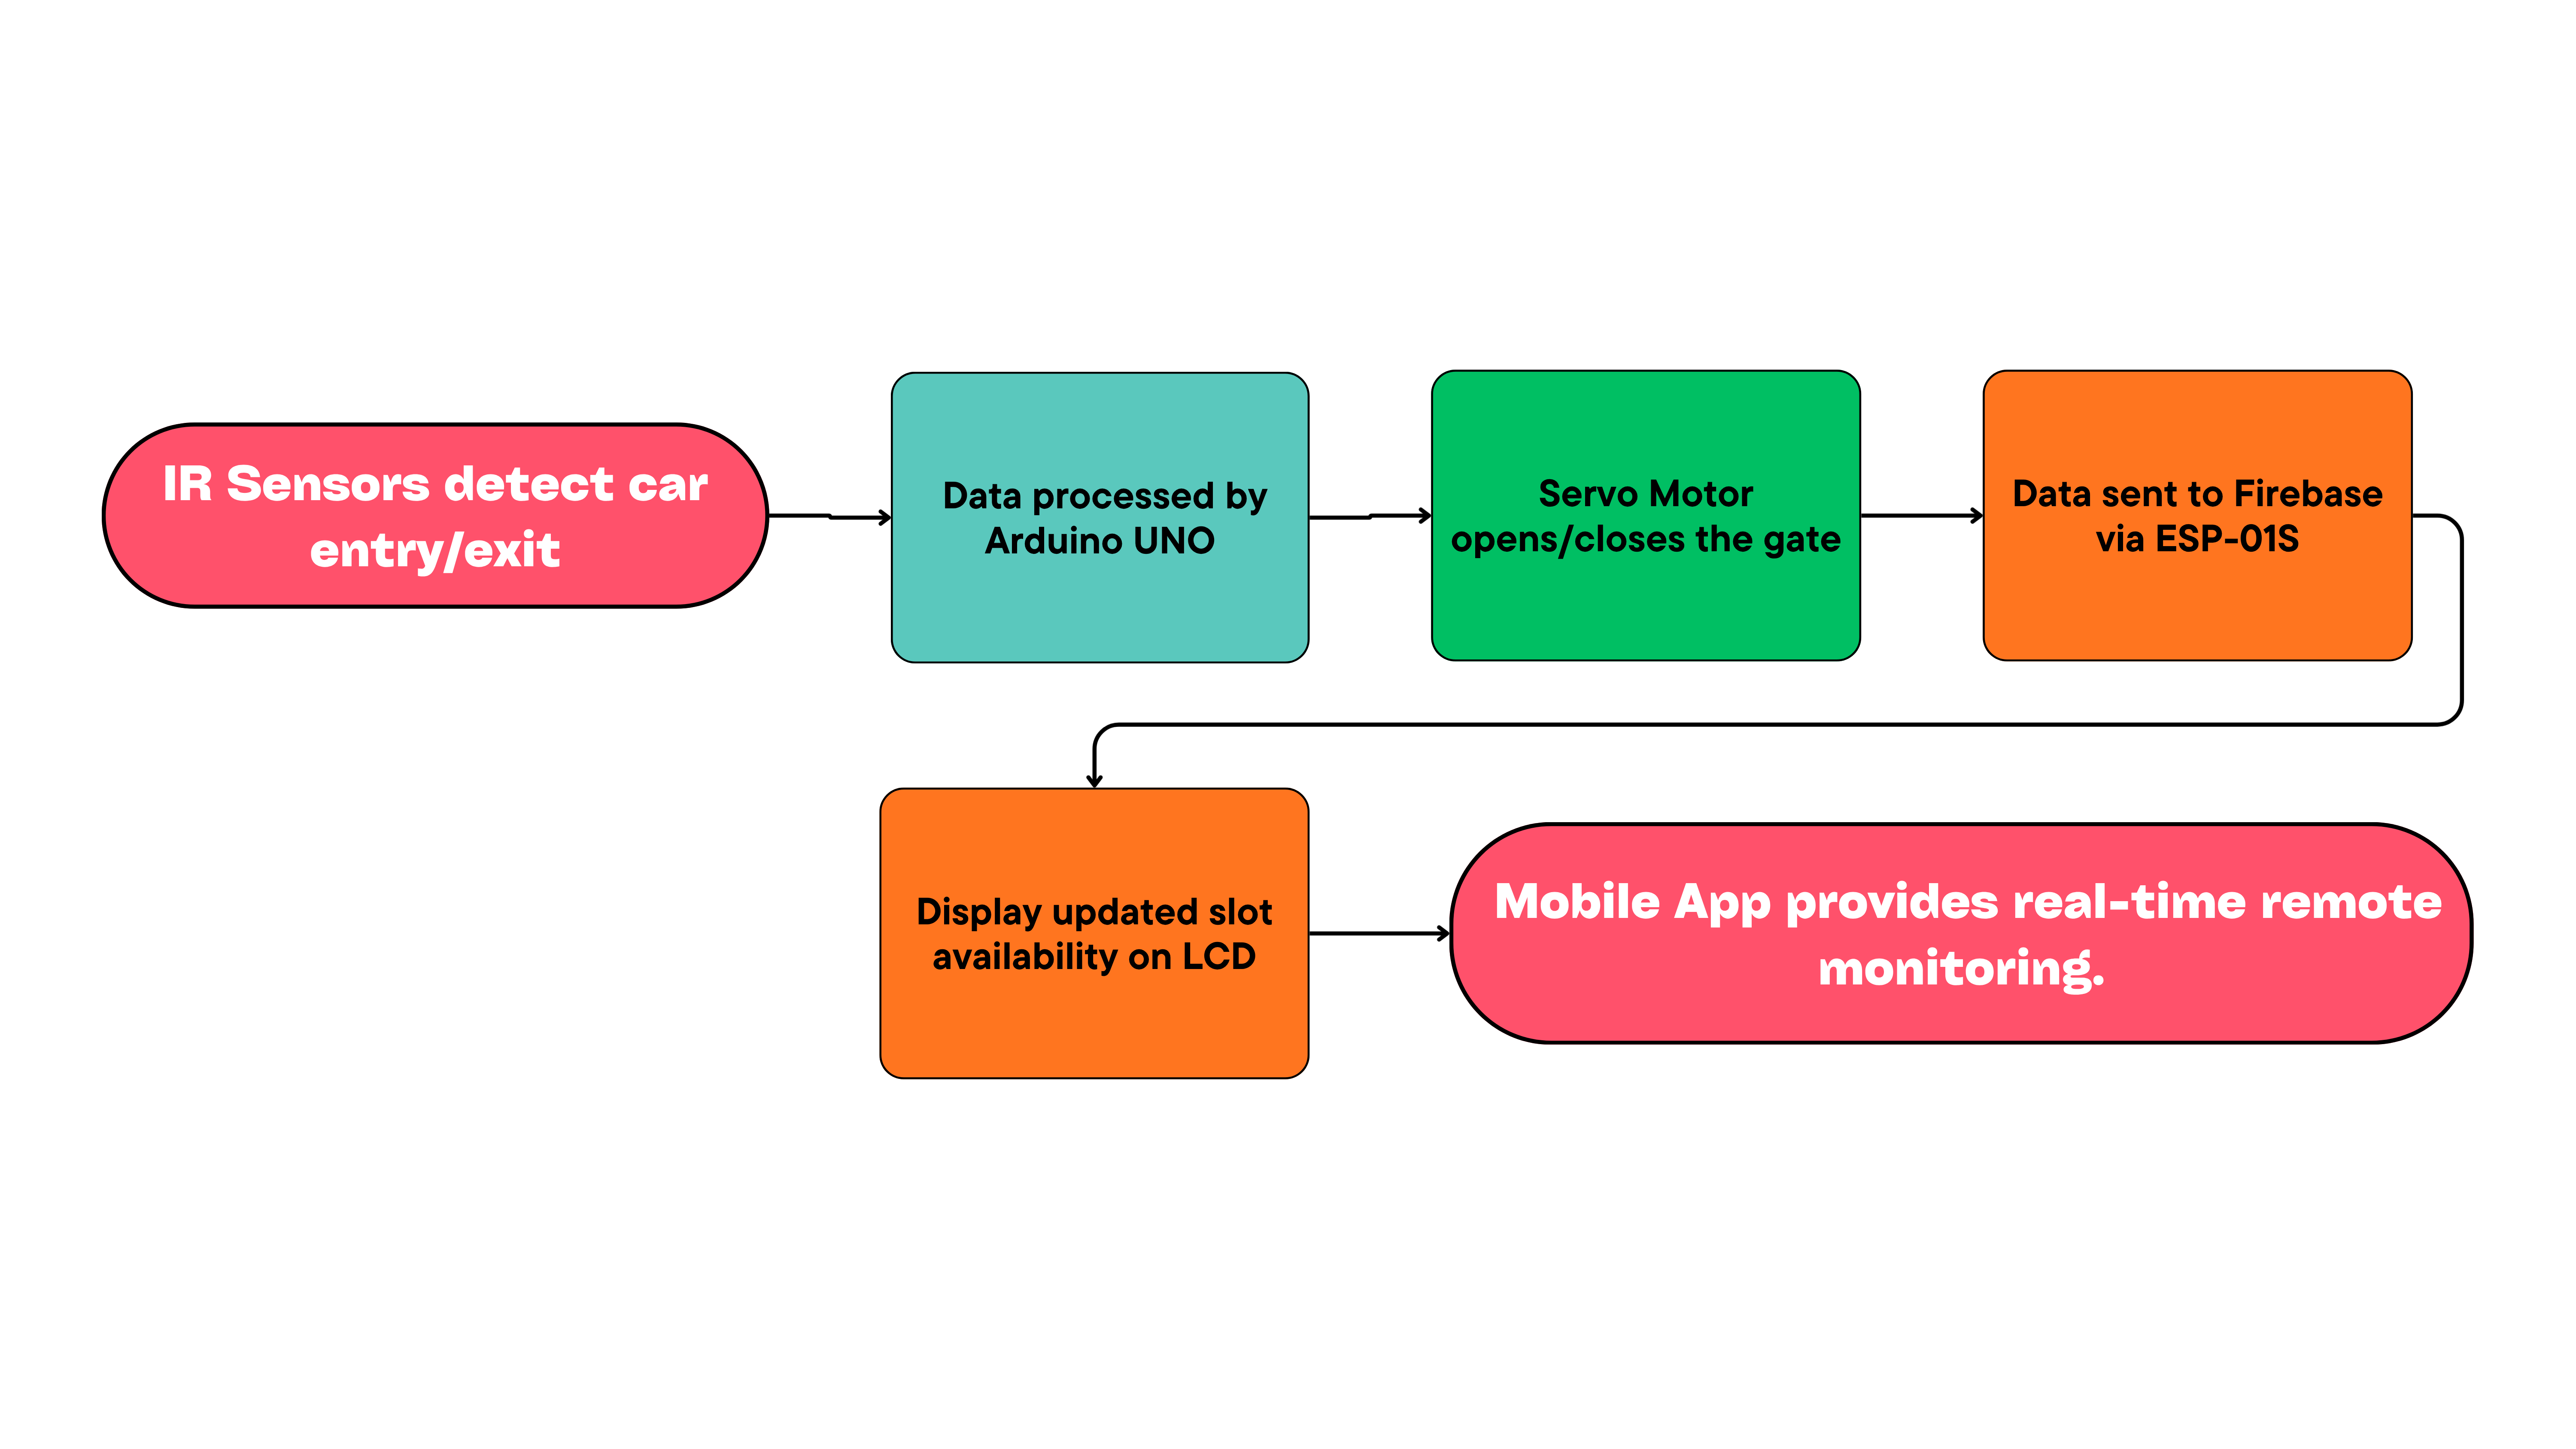
\includegraphics[width=0.78\textwidth]{system_workflow.png}
    \caption{High-Level Workflow of Automated Car Parking System}
    \label{fig:system_workflow}
\end{figure}

\subsection{Embedded System Diagram}

The embedded system diagram in Fig.~\ref{fig:embedded_system_diagram} shows the interaction among the hardware and software modules. The Arduino UNO receives input from the entry IR sensor, exit IR sensor, and RFID reader. It then controls the servo motor-based two-link robotic arm gate, updates the LCD, and communicates with the ESP-01S Wi-Fi module.

The ESP-01S sends parking event data to the middleware server, which stores the information in the online database. The stored data can later be monitored through an online interface or mobile application.

\begin{figure}[H]
    \centering
    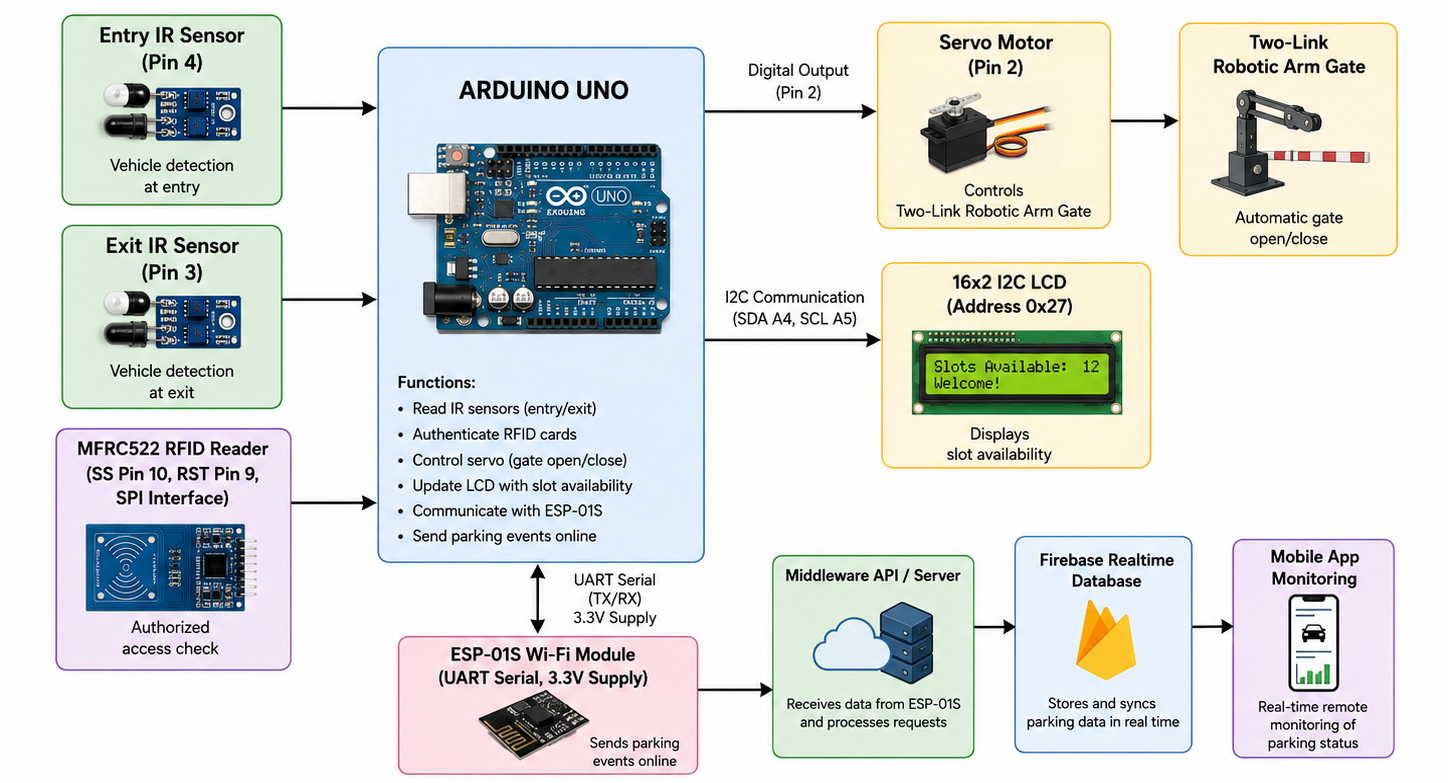
\includegraphics[width=0.82\textwidth]{embedded_car_parking_system_diagram.png}
    \caption{Embedded System Diagram of Automated Car Parking System}
    \label{fig:embedded_system_diagram}
\end{figure}

\section{Hardware Setup}

The hardware setup includes the main electronic and mechanical components required for vehicle detection, authentication, gate control, display, and communication.

\begin{table}[H]
\centering
\small
\caption{Main Hardware Components}
\label{tab:hardware_components}
\begin{tabular}{p{4cm} p{9cm}}
\toprule
\textbf{Component} & \textbf{Function} \\
\midrule
Arduino UNO & Main controller of the system. \\
IR Sensors & Detect vehicle presence at entry and exit points. \\
RFID Module & Reads RFID cards for user authentication. \\
Servo Motor & Controls the two-link robotic arm gate. \\
Two-Link Robotic Arm & Works as the automatic gate mechanism. \\
16x2 I2C LCD & Displays slot availability and system messages. \\
ESP-01S Wi-Fi Module & Sends parking data to the online server or database. \\
Power Supply & Provides required power to the circuit and components. \\
\bottomrule
\end{tabular}
\normalsize
\end{table}

\subsection{Circuit Connection}

The circuit connects all modules with the Arduino UNO. The IR sensors are connected to digital pins for vehicle detection. The RFID module uses SPI communication. The LCD uses I2C communication, which reduces wiring complexity. The servo motor receives control signals from the Arduino, and the ESP-01S communicates through serial AT commands for internet connectivity.

\begin{figure}[H]
    \centering
    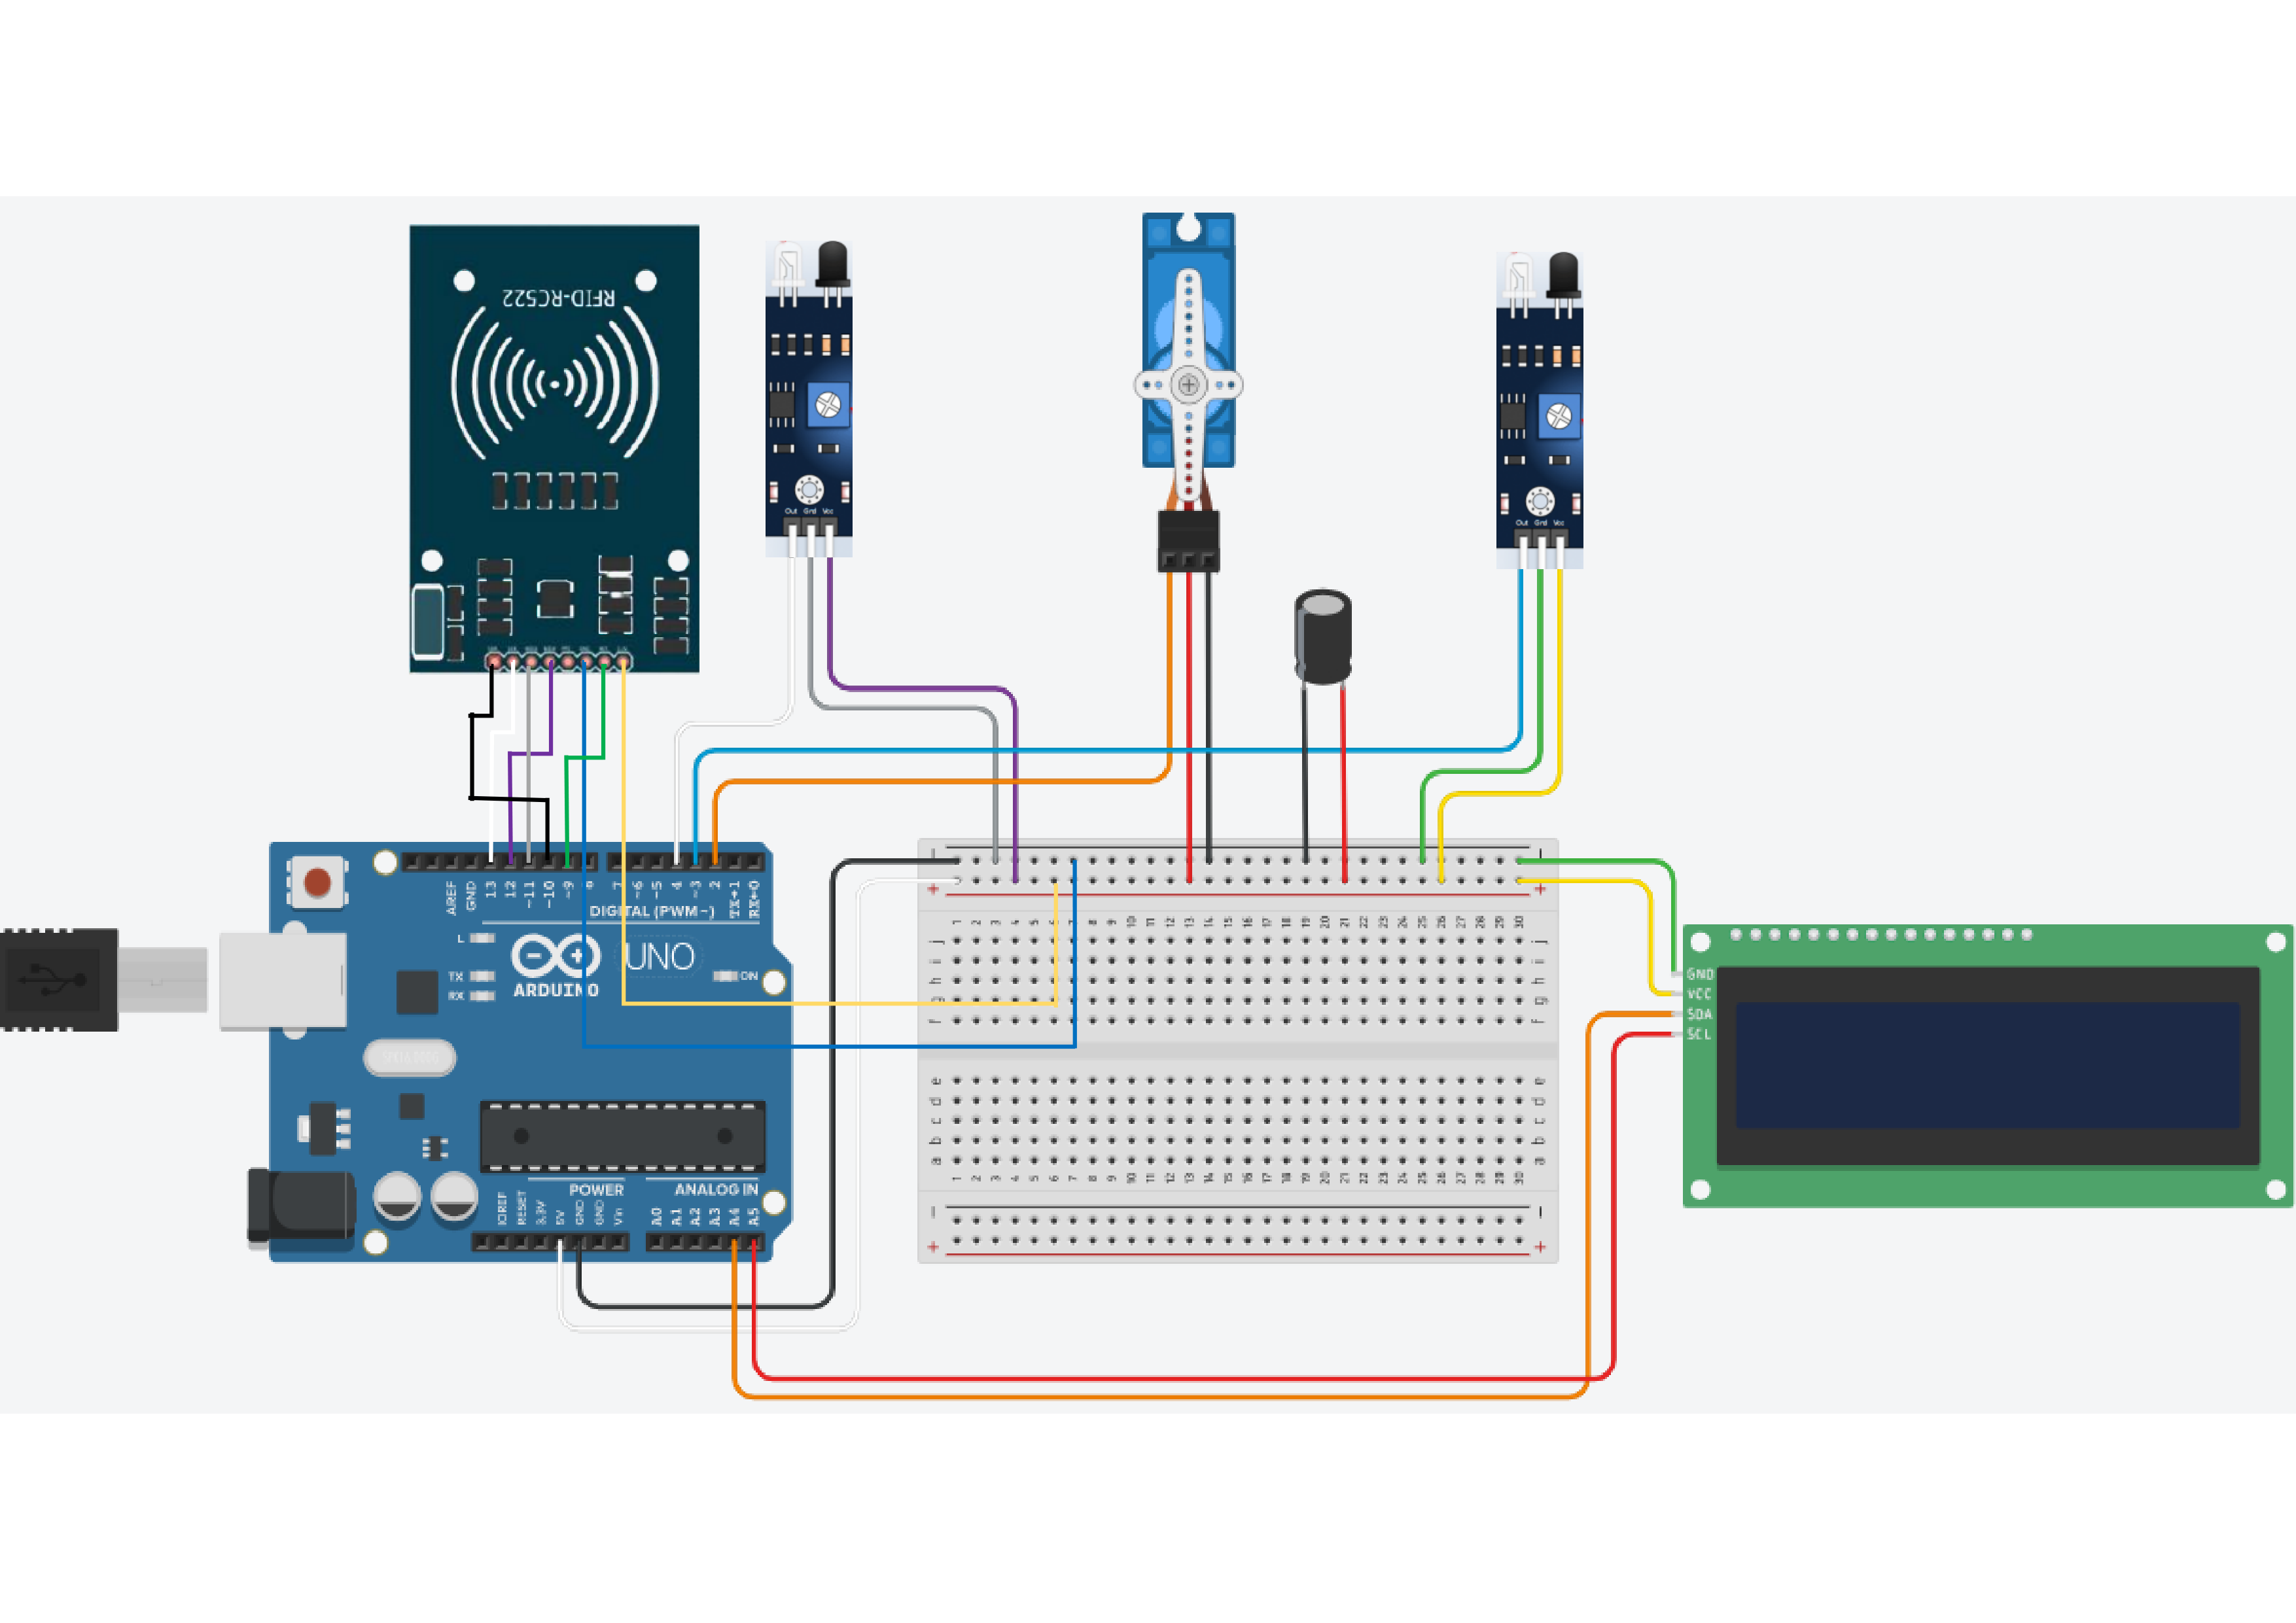
\includegraphics[width=0.78\textwidth]{circuit_connection.png}
    \caption{Circuit Connection of the Proposed System}
    \label{fig:circuit_connection}
\end{figure}

\subsection{Robot Structure Details}

The gate mechanism is designed using a servo motor-controlled two-link robotic arm. The two-link structure provides controlled robotic movement instead of a simple static barrier. When the system grants permission, the servo motor moves the arm to the open position. After the vehicle passes, the arm returns to the closed position.

This structure makes the system suitable for a robotics lab project because it demonstrates actuator control, mechanical movement, and automated response based on sensor input.

\section{Design Alternatives and Rationale}

Several alternatives were considered during design. A manual gate was rejected because it does not provide automation. A simple servo barrier was easier to build but did not demonstrate enough robotic motion. A camera-based system was also considered but would increase cost and complexity.

The final design was selected because it balances cost, functionality, and simplicity. Arduino UNO, IR sensors, RFID, LCD, ESP-01S, and a two-link robotic arm provide a practical solution for a low-cost robotics and IoT-based parking prototype. The design also allows future improvements such as mobile app integration, camera-based vehicle recognition, or payment support.

\section{Summary}

This chapter described the system analysis and design of the Automated Car Parking System. The functional and non-functional requirements, system architecture, embedded system diagram, hardware setup, circuit connection, robotic arm gate mechanism, and design rationale were presented. The selected design is simple, low-cost, and suitable for demonstrating robotics and IoT-based parking automation.



\chapter{Methodology and Implementation}
\label{cha:MethodologyAndImplementationU}

\vspace{-0.8cm}

This chapter describes the methodology and implementation process of the \textbf{Automated Car Parking System}. It explains the development steps, tools, data handling, algorithm, flowchart, and main implementation modules.

\section{Methodological Framework}

The project was developed using a step-by-step embedded system approach. First, the parking problem and required features were identified. Then suitable components were selected based on cost, availability, and compatibility with Arduino UNO. After that, the circuit and robotic arm gate structure were designed. Each module was tested separately and finally integrated into one complete system.

The methodology followed in this project is given below:

\begin{enumerate}
    \item Identify the parking management problem and define objectives.
    \item Select required hardware components.
    \item Design the circuit and two-link robotic arm gate.
    \item Develop Arduino code for sensors, RFID, gate control, LCD, and Wi-Fi communication.
    \item Test each module individually.
    \item Integrate all modules into the final prototype.
    \item Test the system under entry and exit conditions.
\end{enumerate}

\section{Tools, Libraries, and Technologies Used}

The system was developed using both hardware and software tools. Arduino UNO was used as the main controller, and Arduino IDE was used for writing and uploading the program.

\begin{table}[H]
\centering
\small
\caption{Tools, Libraries, and Technologies Used}
\label{tab:tools_technologies}
\begin{tabular}{p{4cm} p{8.5cm}}
\toprule
\textbf{Tool / Technology} & \textbf{Purpose} \\
\midrule
Arduino IDE & Writing, compiling, and uploading Arduino code. \\
Arduino UNO & Main microcontroller of the system. \\
C/C++ & Programming language for Arduino. \\
IR Sensors & Vehicle detection at entry and exit points. \\
MFRC522 RFID Module & RFID card-based authentication. \\
Servo Motor & Controls the two-link robotic arm gate. \\
16x2 I2C LCD & Displays slot availability and system messages. \\
ESP-01S Wi-Fi Module & Sends parking data to the online server. \\
Firebase / Online Database & Stores vehicle entry and exit records. \\
\bottomrule
\end{tabular}
\normalsize
\end{table}

The main Arduino libraries used are \texttt{Wire.h}, \texttt{LiquidCrystal\_I2C.h}, \texttt{Servo.h}, \texttt{SPI.h}, and \texttt{MFRC522.h}. These libraries support I2C communication, LCD control, servo movement, SPI communication, and RFID reading.

\section{Data Collection and Processing}

This project does not use a machine learning dataset. It uses real-time data from hardware modules. The main data includes IR sensor status, RFID UID, slot count, event type, timestamp, and owner information.

\begin{table}[H]
\centering
\small
\caption{System Data Description}
\label{tab:data_description}
\begin{tabular}{p{4cm} p{8.5cm}}
\toprule
\textbf{Data Type} & \textbf{Description} \\
\midrule
IR Sensor Data & Detects vehicle presence at entry or exit. \\
RFID UID & Stores the unique ID of the scanned RFID card. \\
Slot Count & Maintains available parking slots. \\
Event Type & Identifies entry or exit operation. \\
Timestamp & Stores the time of the parking event. \\
Owner Information & Identifies the user linked with the RFID card. \\
\bottomrule
\end{tabular}
\normalsize
\end{table}

The Arduino processes the collected data. RFID UID is converted into a readable string, trimmed, and matched with authorized UID values. The system also prepares a timestamp and checks the slot count to avoid invalid updates. For every valid entry or exit, a JSON packet is created and sent online through the ESP-01S Wi-Fi module.

\section{Model Development / Algorithm Design}

The project does not use a machine learning model. It follows rule-based control logic. The Arduino continuously checks the entry and exit IR sensors. If a vehicle is detected at the entry point, the system checks slot availability and requests RFID authentication. If the RFID card is valid, the gate opens and the slot count is updated.

\subsection{System Flowchart}

Fig.~\ref{fig:flowchart_diagram} shows the working flow of the Automated Car Parking System. It includes hardware initialization, vehicle detection, slot checking, RFID verification, robotic arm gate control, LCD update, and online data transmission.

\begin{figure}[H]
    \centering
    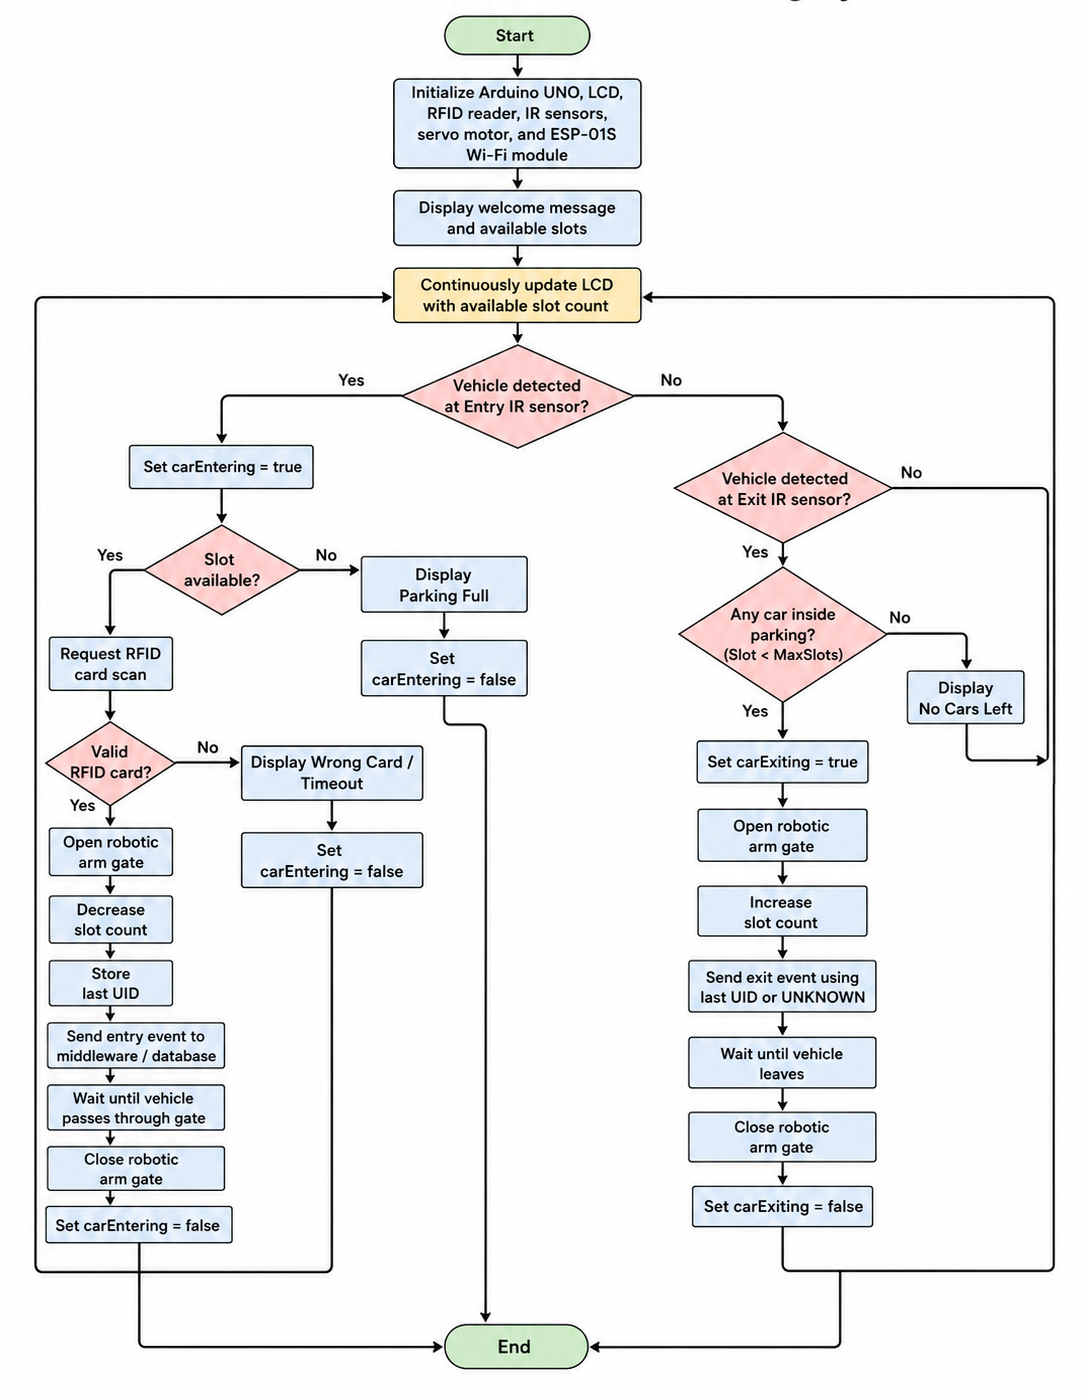
\includegraphics[height=0.72\textheight]{flowchart_of_automated_car_parking_system.png}
    \caption{Flowchart of Automated Car Parking System}
    \label{fig:flowchart_diagram}
\end{figure}

The simplified algorithm is given below:

\begin{algorithm}[H]
\caption{System Operation Algorithm}
\begin{algorithmic}[1]
\State Initialize LCD, RFID, servo motor, IR sensors, and Wi-Fi module
\State Set maximum parking slot value
\While{system is active}
    \If{entry sensor detects a car}
        \If{slot is available}
            \State Request RFID card scan
            \If{RFID card is valid}
                \State Open robotic arm gate
                \State Decrease slot count
                \State Send entry data to online server
                \State Close robotic arm gate
            \Else
                \State Display access denied message
            \EndIf
        \Else
            \State Display parking full message
        \EndIf
    \EndIf

    \If{exit sensor detects a car}
        \State Open robotic arm gate
        \State Increase slot count
        \State Send exit data to online server
        \State Close robotic arm gate
    \EndIf

    \State Update LCD display
\EndWhile
\end{algorithmic}
\end{algorithm}

\section{System Implementation / Modules Description}

The system was implemented by dividing it into functional modules. Each module performs a specific task and communicates with the Arduino UNO.

\subsection{Vehicle Detection Module}

Two IR sensors are used to detect vehicles at the entry and exit points. When a vehicle is detected, the sensor sends a digital signal to the Arduino and starts the entry or exit process.

\subsection{RFID Authentication Module}

The RFID module checks whether the user is authorized. If the scanned card matches a stored UID, the system allows entry. Otherwise, the LCD displays a wrong card or access denied message.

\subsection{Robotic Arm Gate Module}

The gate is controlled by a servo motor connected to a two-link robotic arm. When entry or exit is allowed, the servo moves the arm to the open position. After the vehicle passes, the arm returns to the closed position. Smooth movement is created by changing the servo angle step by step.

\subsection{LCD Display Module}

The 16x2 I2C LCD displays welcome messages, RFID scanning messages, wrong card alerts, parking full messages, gate status, and available slot count. This helps users understand the current system condition.

\subsection{IoT Communication Module}

The ESP-01S Wi-Fi module sends parking data to the online server using AT commands. For each valid event, the Arduino creates a JSON message and sends it through an HTTP POST request.

\begin{lstlisting}
{
  "uid": "F6 A9 23 03",
  "event": "entry",
  "owner": "MRJ",
  "timestamp": "00:05:23"
}
\end{lstlisting}

\section{Hardware and Software Requirements}

\begin{table}[H]
\centering
\small
\caption{Hardware and Software Requirements}
\label{tab:hardware_software_req}
\begin{tabular}{p{4cm} p{8.5cm}}
\toprule
\textbf{Category} & \textbf{Requirements} \\
\midrule
Controller & Arduino UNO \\
Sensors & Two IR sensors for entry and exit detection \\
Authentication & MFRC522 RFID reader and RFID cards \\
Actuator & Servo motor with two-link robotic arm mechanism \\
Display & 16x2 I2C LCD display \\
Communication & ESP-01S Wi-Fi module \\
Power Supply & 5V supply for Arduino and connected modules \\
Programming Tool & Arduino IDE \\
Programming Language & C/C++ for Arduino \\
Libraries & Wire, LiquidCrystal\_I2C, Servo, SPI, MFRC522 \\
Online Platform & Online server or database for parking data storage \\
\bottomrule
\end{tabular}
\normalsize
\end{table}

\section{Summary}

This chapter explained the methodology and implementation of the Automated Car Parking System. It described the development steps, tools, system data, processing method, flowchart, algorithm, implementation modules, and hardware-software requirements. The final implementation combines vehicle detection, RFID authentication, robotic arm gate control, LCD display, and IoT-based data transmission.



\chapter{Results and Evaluation}
\label{cha:ResultsAndEvaluationU}

\vspace{-0.8cm}

This chapter presents the results and evaluation of the \textbf{Automated Car Parking System}. The system was tested to evaluate vehicle detection, RFID authentication, robotic arm gate movement, parking slot update, LCD output, and IoT data transmission.

\section{Experimental Setup}

The prototype was tested in a lab environment using a small-scale parking model. The setup included Arduino UNO, two IR sensors, MFRC522 RFID module, servo motor, two-link robotic arm gate, 16x2 I2C LCD, and ESP-01S Wi-Fi module. Toy cars or hand-based object movement were used to simulate vehicle entry and exit.

The entry IR sensor was placed near the entrance gate, and the exit IR sensor was placed near the exit point. The RFID reader was placed at the entrance for authorized access. The servo motor controlled the robotic arm gate, the LCD displayed available slots, and the Wi-Fi module sent parking records to the online server.

\begin{table}[H]
\centering
\small
\caption{Experimental Setup}
\label{tab:experimental_setup}
\begin{tabular}{p{4cm} p{8.5cm}}
\toprule
\textbf{Item} & \textbf{Description} \\
\midrule
Controller & Arduino UNO \\
Vehicle Detection & IR sensors at entry and exit points \\
Authentication & MFRC522 RFID reader and RFID cards \\
Gate Mechanism & Servo motor-controlled two-link robotic arm \\
Display Unit & 16x2 I2C LCD display \\
Communication & ESP-01S Wi-Fi module \\
Parking Capacity & 4 prototype parking slots \\
Testing Method & Repeated entry and exit simulation \\
\bottomrule
\end{tabular}
\normalsize
\end{table}

\section{Performance Evaluation}

The system was evaluated based on functional correctness, response behavior, and module reliability. The main testing areas were vehicle detection, RFID verification, gate operation, slot count update, LCD display, and IoT data transmission.

\begin{table}[H]
\centering
\small
\caption{Functional Test Result}
\label{tab:functional_test_result}
\begin{tabular}{p{4.6cm} p{2.2cm} p{2.2cm} p{3cm}}
\toprule
\textbf{Test Case} & \textbf{Total Test} & \textbf{Successful} & \textbf{Result} \\
\midrule
Entry IR detection & 20 & 20 & Successful \\
Exit IR detection & 20 & 20 & Successful \\
Valid RFID detection & 15 & 15 & Successful \\
Invalid RFID rejection & 10 & 10 & Successful \\
Robotic arm gate operation & 20 & 19 & Mostly successful \\
Parking slot update & 20 & 20 & Successful \\
LCD status display & 20 & 20 & Successful \\
IoT data transmission & 20 & 18 & Mostly successful \\
\bottomrule
\end{tabular}
\normalsize
\end{table}

The test results show that the IR sensors detected vehicles accurately during prototype testing. RFID authentication worked correctly for both valid and invalid cards. The robotic arm gate opened and closed successfully in most cases, although minor movement variation occurred due to servo positioning and mechanical alignment. The LCD displayed correct slot information, and IoT data transmission was successful in most tests, depending on Wi-Fi stability.

\begin{table}[H]
\centering
\small
\caption{Overall Performance Summary}
\label{tab:overall_performance}
\begin{tabular}{p{5cm} p{4cm} p{3.5cm}}
\toprule
\textbf{Performance Area} & \textbf{Observed Performance} & \textbf{Comment} \\
\midrule
Vehicle Detection & 100\% & Accurate in lab testing \\
RFID Authentication & 100\% & Valid and invalid cards detected correctly \\
Robotic Arm Operation & 95\% & Minor adjustment needed \\
Slot Count Update & 100\% & Updated correctly \\
LCD Display & 100\% & Displayed correct status \\
IoT Data Transmission & 90\% & Depended on Wi-Fi connection \\
\bottomrule
\end{tabular}
\normalsize
\end{table}

\section{Discussion on Findings}

The experimental results indicate that the main objectives of the project were achieved. The system successfully detected vehicle presence, verified RFID cards, controlled the two-link robotic arm gate, updated parking slot count, displayed information on the LCD, and sent data to the online server.

Compared with a manual parking system, the proposed system reduces human involvement in gate control, slot counting, and record keeping. Compared with a simple servo gate system, this project adds RFID authentication, IoT-based data storage, and a two-link robotic arm mechanism, making it more suitable for robotics lab demonstration.

The IR sensors performed well at short range, and RFID provided a simple and effective access control method. The servo motor controlled the robotic arm properly, but mechanical alignment was important for smooth movement. The IoT module added remote record storage, although its performance depended on Wi-Fi connection quality and ESP-01S response time.

\section{Limitations}

Although the prototype performed successfully, it has some limitations. The system was tested on a small-scale model, so real-world implementation would require a stronger motor, better mechanical structure, and more durable materials. IR sensors may be affected by object position, distance, or lighting conditions. The robotic arm also needs proper alignment for stable movement.

The Wi-Fi communication depends on network availability. If the connection is weak, online data transmission may fail. The current prototype uses RFID only and does not include automatic number plate recognition, mobile application, payment system, camera-based detection, or large-scale database management.

\section{Summary}

This chapter presented the experimental setup, functional test results, performance summary, discussion, and limitations of the Automated Car Parking System. The results show that the system can perform vehicle detection, RFID authentication, robotic arm gate control, slot count update, LCD display, and IoT data transmission successfully. Overall, the project demonstrates a practical prototype of a robotics and IoT-based automated parking system.



\chapter{Project Planning and Budget}
\label{cha:cost_time}

\vspace{-0.8cm}

This chapter presents the project planning and budget estimation of the \textbf{Automated Car Parking System}. It shows the project timeline, required resources, and estimated cost for completing the prototype.

\section{Project Timeline}

The project was completed through requirement analysis, component selection, system design, hardware setup, coding, testing, integration, documentation, and presentation preparation. The eight-week timeline helped the team divide tasks properly and complete the project in an organized way.

\begin{table}[H]
\centering
\small
\renewcommand{\arraystretch}{1.15}
\caption{Eight-Week Project Timeline}
\label{tab:gantt_chart}
\resizebox{\textwidth}{!}{
\begin{tabular}{|p{4.2cm}|c|c|c|c|c|c|c|c|}
\hline
\textbf{Project Phase} & \textbf{W1} & \textbf{W2} & \textbf{W3} & \textbf{W4} & \textbf{W5} & \textbf{W6} & \textbf{W7} & \textbf{W8} \\
\hline
Requirement Analysis & \cellcolor{gray!40} &  &  &  &  &  &  &  \\
\hline
Component Selection & \cellcolor{gray!40} & \cellcolor{gray!40} &  &  &  &  &  &  \\
\hline
System Design &  & \cellcolor{gray!40} & \cellcolor{gray!40} &  &  &  &  &  \\
\hline
Circuit and Hardware Setup &  &  & \cellcolor{gray!40} & \cellcolor{gray!40} &  &  &  &  \\
\hline
Arduino Coding &  &  &  & \cellcolor{gray!40} & \cellcolor{gray!40} &  &  &  \\
\hline
Module Testing &  &  &  &  & \cellcolor{gray!40} & \cellcolor{gray!40} &  &  \\
\hline
Final Integration &  &  &  &  &  & \cellcolor{gray!40} & \cellcolor{gray!40} &  \\
\hline
Testing and Validation &  &  &  &  &  &  & \cellcolor{gray!40} & \cellcolor{gray!40} \\
\hline
Report Writing and Presentation &  &  &  &  &  & \cellcolor{gray!40} & \cellcolor{gray!40} & \cellcolor{gray!40} \\
\hline
\end{tabular}
}
\normalsize
\end{table}

The project followed the planned timeline closely. Extra attention was needed during hardware integration because the two-link robotic arm gate required proper mechanical alignment for smooth movement.

\section{Budget Estimation}

The budget was estimated based on the required hardware components and supporting materials. Most software tools used in this project were free.

\begin{table}[H]
\centering
\small
\renewcommand{\arraystretch}{1.15}
\caption{Estimated Project Budget}
\label{tab:project_budget}
\begin{tabular}{|p{0.38\textwidth}|p{0.13\textwidth}|p{0.18\textwidth}|p{0.18\textwidth}|}
\hline
\textbf{Item / Resource} & \textbf{Qty.} & \textbf{Unit Cost} & \textbf{Total Cost} \\
\hline
Arduino UNO & 1 & 700 & 700 \\
\hline
MFRC522 RFID Module with Card & 1 Set & 250 & 250 \\
\hline
IR Sensors & 2 & 100 & 200 \\
\hline
Servo Motor & 1 & 250 & 250 \\
\hline
ESP-01S Wi-Fi Module & 1 & 300 & 300 \\
\hline
16x2 I2C LCD Display & 1 & 350 & 350 \\
\hline
Breadboard and Jumper Wires & 1 Set & 250 & 250 \\
\hline
Robotic Arm / Gate Materials & 1 Set & 400 & 400 \\
\hline
Power Supply and Connectors & 1 Set & 300 & 300 \\
\hline
Printing and Presentation Materials & - & 300 & 300 \\
\hline
\textbf{Total Estimated Budget} &  &  & \textbf{3,300 BDT} \\
\hline
\end{tabular}
\normalsize
\end{table}

The total estimated cost of the project was approximately \textbf{3,300 BDT}. The cost may vary depending on component quality and market availability.

\section{Software and Service Cost}

The software tools and online services were used in free or prototype-accessible versions.

\begin{table}[H]
\centering
\small
\renewcommand{\arraystretch}{1.15}
\caption{Software and Service Cost}
\label{tab:software_budget}
\begin{tabular}{|p{0.4\textwidth}|p{0.3\textwidth}|p{0.18\textwidth}|}
\hline
\textbf{Software / Service} & \textbf{Purpose} & \textbf{Cost} \\
\hline
Arduino IDE & Code development and upload & Free \\
\hline
Arduino Libraries & LCD, RFID, Servo, and SPI support & Free \\
\hline
Online Database / Server & Parking data storage & Free / Prototype Use \\
\hline
GitHub Repository & Code and report submission & Free \\
\hline
\end{tabular}
\normalsize
\end{table}

\section{Summary}

This chapter presented the eight-week project timeline and estimated budget of the Automated Car Parking System. The project was completed through planning, hardware setup, coding, testing, integration, and documentation phases. The budget shows that the system can be developed using low-cost hardware and free software tools, making it feasible for academic prototype implementation.



\chapter{Standards and Design Constraints}
\label{cha:AccreditationComponents}

\vspace{-0.8cm}

This chapter discusses how the \textbf{Automated Car Parking System} satisfies engineering standards, design constraints, Complex Engineering Problem (CEP) attributes, Complex Engineering Activity (CEA) attributes, and Knowledge Profile requirements. Since the project combines hardware, software, robotics, and IoT communication, safety, reliability, privacy, sustainability, and professional responsibility were considered during design and implementation.

\section{Compliance with Standards and Professional Practice}

The project followed basic engineering practices for embedded system design, hardware interfacing, modular programming, IoT communication, documentation, and testing. Relevant documentation such as Arduino UNO, Servo library, MFRC522 RFID module, ESP8266, and Firebase documentation was considered during development \cite{b8,b9,b10,b11,b12}.

\subsection{Software and Hardware Practice}

The software was developed using Arduino C/C++ in Arduino IDE. The code was organized into separate functions for RFID reading, gate control, LCD update, Wi-Fi connection, timestamp generation, and data transmission. Standard libraries such as \texttt{Servo.h}, \texttt{SPI.h}, \texttt{MFRC522.h}, \texttt{Wire.h}, and \texttt{LiquidCrystal\_I2C.h} were used.

The hardware design followed basic low-voltage embedded system interfacing practice. Arduino UNO was used as the controller, IR sensors were used for detection, MFRC522 used SPI communication, LCD used I2C communication, ESP-01S used serial communication, and the servo motor controlled the two-link robotic arm. Safe testing was performed using a small-scale prototype instead of a real vehicle gate.

\subsection{Professional Considerations}

The system stores RFID UID, entry/exit event, owner information, and timestamp. Therefore, privacy and responsible data use were considered. In real deployment, Wi-Fi credentials, database keys, and user records must be protected and should not be published in source code or reports.

\section{Design Constraints}

The project was affected by cost, component availability, sensor accuracy, power stability, mechanical alignment, and Wi-Fi reliability. Since it was developed as an academic prototype, low-cost components were selected while keeping the main functions operational.

\subsection{Ethical, Safety, and Sustainability Considerations}

The testing results and limitations were reported honestly. Related works and technical documentation were cited properly. RFID and online data should be handled responsibly to protect user privacy.

For safety, low-voltage components were used and the robotic arm was tested in a controlled lab environment. The servo movement was kept smooth to reduce sudden motion, and direct contact with the moving arm was avoided during operation.

From an environmental perspective, the system uses low-power and reusable electronic components. In practical use, automated parking can reduce unnecessary waiting time and vehicle movement near the gate, which may help reduce fuel consumption and emissions.

\section{Complex Engineering Problem (CEP) Coverage}

The project addresses a complex engineering problem because it integrates embedded control, sensors, authentication, robotic actuation, IoT communication, and real-time decision making.

\begin{table}[H]
\centering
\small
\caption{Mapping with Complex Engineering Problems (Ps)}
\label{tab:cep_mapping}
\resizebox{\textwidth}{!}{
\begin{tabular}{|p{0.07\textwidth}|p{0.24\textwidth}|p{0.5\textwidth}|p{0.17\textwidth}|}
\hline
\textbf{Ps} & \textbf{Attributes} & \textbf{How Ps are addressed} & \textbf{Evidence} \\
\hline
P1 & Depth of Knowledge & Applies embedded systems, sensors, RFID, servo control, IoT, and database communication. & Ch. 2, 3, 4 \\
\hline
P2 & Conflicting Requirements & Balances low cost, real-time response, reliable detection, smooth gate movement, and online data transfer. & Ch. 3, 5 \\
\hline
P3 & Depth of Analysis & Analyzes sensor response, RFID validation, slot counting, robotic arm motion, and Wi-Fi transmission. & Ch. 4, 5 \\
\hline
P4 & Familiarity of Issues & Parking automation is known, but robotic arm gate with IoT monitoring creates project-specific challenges. & Ch. 1, 2, 3 \\
\hline
P5 & Applicable Standards & Uses standard Arduino libraries, hardware interfacing practices, and IoT data handling principles. & Sec. 7.1 \\
\hline
P6 & Stakeholder Needs & Supports drivers, parking managers, and maintainers through automation and monitoring. & Ch. 3, Appendix \\
\hline
P7 & Interdependence & Sensors, RFID, servo, LCD, Wi-Fi, and server are interconnected; failure of one module affects the system. & Ch. 3, 4, 5 \\
\hline
\end{tabular}
}
\normalsize
\end{table}

\section{Complex Engineering Activities (CEA) Coverage}

The project involves complex engineering activities because it required multiple resources, hardware-software interaction, implementation, testing, and evaluation.

\begin{table}[H]
\centering
\small
\caption{Mapping of Complex Engineering Activities (As)}
\label{tab:activities_mapping}
\resizebox{\textwidth}{!}{
\begin{tabular}{|p{0.07\textwidth}|p{0.24\textwidth}|p{0.5\textwidth}|p{0.17\textwidth}|}
\hline
\textbf{As} & \textbf{Attributes} & \textbf{How As are addressed} & \textbf{Evidence} \\
\hline
A1 & Range of Resources & Uses Arduino UNO, IR sensors, RFID, ESP-01S, LCD, servo motor, robotic arm materials, libraries, and online database. & Ch. 3, 4 \\
\hline
A2 & Level of Interaction & Multiple modules interact, including sensors, RFID, servo, LCD, Wi-Fi module, and server. & Ch. 3, 4 \\
\hline
A3 & Innovation & Uses a two-link robotic arm gate instead of a simple static barrier. & Ch. 3, 5 \\
\hline
A4 & Society and Environment & Can reduce waiting time, improve parking management, reduce manual effort, and support smart city applications. & Ch. 1, 7 \\
\hline
A5 & Familiarity & Combines known technologies into a practical robotics-IoT parking automation prototype. & Ch. 2, 4 \\
\hline
\end{tabular}
}
\normalsize
\end{table}

\section{Knowledge Profile Mapping}

\begin{table}[H]
\centering
\small
\caption{Knowledge Profile Mapping}
\label{tab:knowledge_profile_mapping}
\resizebox{\textwidth}{!}{
\begin{tabular}{|p{0.09\textwidth}|p{0.35\textwidth}|p{0.48\textwidth}|}
\hline
\textbf{Profile} & \textbf{Knowledge Area} & \textbf{Project Evidence} \\
\hline
K1 & Natural science and engineering fundamentals & Sensor detection, electrical interfacing, and servo control. \\
\hline
K2 & Mathematics and computing & Control logic, slot counting, timestamp generation, and data formatting. \\
\hline
K3 & Engineering fundamentals & Embedded system design using Arduino and electronic modules. \\
\hline
K4 & Specialist knowledge & RFID authentication, IoT communication, and robotic arm gate control. \\
\hline
K5 & Engineering design & System architecture, circuit design, and hardware-software integration. \\
\hline
K6 & Engineering practice & Prototype development, testing, debugging, and documentation. \\
\hline
K7 & Social, environmental, and safety knowledge & Parking efficiency, safety, data privacy, and sustainability considerations. \\
\hline
K8 & Research literature and standards & Related works review and use of technical documentation. \\
\hline
\end{tabular}
}
\normalsize
\end{table}

\section{Summary}

This chapter presented the standards, design constraints, CEP coverage, CEA coverage, and Knowledge Profile mapping of the Automated Car Parking System. The project satisfies engineering requirements by integrating embedded control, robotics, IoT communication, and real-time parking management while considering safety, privacy, sustainability, and professional responsibility.



\chapter{Conclusion and Future Work}
\label{cha:ConclusionAndFutureWork}

\vspace{-0.8cm}

This chapter presents the conclusion of the \textbf{Automated Car Parking System} project. It summarizes the completed work, key findings, limitations, and possible future improvements.

\section{Summary of the Work}

The main objective of this project was to design and implement an Automated Car Parking System using robotics and IoT technologies. The system was developed using Arduino UNO, IR sensors, RFID module, ESP-01S Wi-Fi module, 16x2 I2C LCD display, servo motor, and a two-link robotic arm gate mechanism.

The system detects vehicles at the entry and exit points using IR sensors. During entry, it checks slot availability and verifies the RFID card before opening the gate. If the RFID card is valid and a slot is available, the servo motor moves the two-link robotic arm to open the gate. After vehicle entry, the slot count is updated on the LCD and the entry record is sent to the online server. During exit, the system opens the gate, updates the slot count, and sends the exit record online.

The final prototype was tested in a lab environment and performed successfully in vehicle detection, RFID authentication, robotic arm gate operation, slot count update, LCD display, and IoT-based data transmission.

\section{Key Findings and Contributions}

The project achieved its major objectives and produced a functional prototype. The key findings and contributions are listed below:

\begin{itemize}
    \item IR sensors successfully detected vehicles at entry and exit points.
    \item RFID authentication allowed only authorized users to enter.
    \item The servo motor-controlled two-link robotic arm worked as an automatic gate.
    \item The LCD displayed real-time parking slot availability and system messages.
    \item The ESP-01S Wi-Fi module transmitted entry and exit records online.
    \item The system reduced manual gate control, slot counting, and record keeping.
    \item The project demonstrated practical integration of robotics and IoT in parking automation.
\end{itemize}

The main technical contribution of the project is the use of a two-link robotic arm gate instead of a simple static barrier. This makes the system more suitable for a robotics-based automation project.

\section{Limitations of the Study}

Although the system worked successfully as a prototype, it has some limitations. The system was tested on a small-scale model, so real-world implementation would require stronger motors, durable materials, and improved mechanical structure. IR sensors may be affected by object position, distance, and surrounding conditions. The robotic arm also requires proper alignment for stable movement.

The Wi-Fi communication depends on network availability, so weak internet connection may delay or stop online data transmission. The current system uses RFID-based authentication only and does not include automatic number plate recognition, mobile application, payment system, reservation system, or camera-based detection.

\section{Recommendations and Future Work}

The prototype can be improved in several ways. Future improvements may include:

\begin{itemize}
    \item Adding automatic number plate recognition using a camera.
    \item Developing a mobile application for users and administrators.
    \item Adding online parking reservation and payment features.
    \item Improving data security for RFID records and online communication.
    \item Using stronger motors and durable materials for real gate operation.
    \item Adding backup power support for continuous operation.
    \item Improving the robotic arm design for smoother movement.
    \item Adding individual slot sensors for multiple parking spaces.
\end{itemize}

In conclusion, the Automated Car Parking System successfully fulfills the main goal of automating parking entry and exit using robotics and IoT technologies. The project provides a practical prototype that can be further improved for academic, residential, and commercial parking environments.



% ---------------- References ----------------
\bibliographystyle{plain}
\bibliography{references.bib}

% ---------------- Appendices ----------------
\appendix

\chapter*{Appendices}
\markboth{Appendices}{}
\addcontentsline{toc}{chapter}{Appendices}

\setcounter{section}{0}
\renewcommand{\thesection}{\Alph{section}}

\section{Source Code / GitHub Link}

The complete source code, final report PDF, diagrams, and relevant resources of the \textbf{Automated Car Parking System} will be uploaded to a GitHub repository for documentation and replication purposes.

\textbf{GitHub Repository Link:} \\
\url{https://github.com/Mamim57/Automated-Car-Parking-System}

The main Arduino source code file is:

\begin{itemize}
    \item \texttt{Robo\_Car\_Parking.ino}
\end{itemize}

The source code includes IR sensor reading, RFID authentication, LCD update, servo motor-based robotic arm gate control, parking slot counting, and ESP-01S Wi-Fi based data transmission.

For security reasons, sensitive information such as Wi-Fi SSID, Wi-Fi password, API keys, and database credentials should not be published directly. These values should be replaced with placeholders before public submission.

\begin{lstlisting}
String ssid = "YOUR_WIFI_NAME";
String password = "YOUR_WIFI_PASSWORD";
\end{lstlisting}

\section{Team Responsibilities}

\begin{table}[H]
\centering
\small
\renewcommand{\arraystretch}{1.15}
\caption{Team Member Responsibilities}
\label{tab:team_responsibilities}
\begin{tabular}{|p{4cm}|p{9cm}|}
\hline
\textbf{Team Member} & \textbf{Contribution} \\
\hline
Md. Mizanur Rahman & Arduino coding, system logic, Firebase/online database setup, Wi-Fi data communication, and software debugging. \\
\hline
Md. Shahid Al Mamim & Hardware setup, component selection, circuit connection, robotic arm gate setup, system testing, and report writing. \\
\hline
Lamia Akter Jesmin & Survey preparation, system analysis, requirement analysis, report writing, and Wi-Fi module integration support. \\
\hline
\end{tabular}
\normalsize
\end{table}

\section{Ethics and Compliance Statements}

The project was developed for academic and prototype demonstration purposes. The survey data was used only for academic research, and personal information was not shared in the report. RFID and parking event data were used only for system testing.

The following ethical issues were considered:

\begin{itemize}
    \item Testing results were reported honestly.
    \item Related works and technical documents were cited properly.
    \item Wi-Fi passwords, API keys, and database credentials were kept private.
    \item The robotic arm gate was tested safely in a controlled lab environment.
    \item RFID and parking event data were used only for project demonstration.
\end{itemize}

In a real deployment, proper data privacy, secure communication, and user consent should be maintained.

\section{Survey 1: Initial User Need Analysis}

The first survey was conducted to understand user perception about the product concept and its possible usefulness. During the initial concept discussion, both automated car parking and an expression bot idea were mentioned. However, the final implemented project focused only on the \textbf{Automated Car Parking System}. Therefore, the expression bot was treated as an early brainstorming idea and was not included in the final implementation.

\subsection*{Survey Questions}

\begin{enumerate}
    \item What is your job role?
    \item Are you involved in purchasing or decision making?
    \item Have you understood the product concept?
    \item Do you think the product will be helpful for your workplace?
    \item Do you have any additional comments?
\end{enumerate}

\subsection*{Survey Response Summary}

\begin{table}[H]
\centering
\small
\renewcommand{\arraystretch}{1.15}
\caption{Summary of Survey 1 Response}
\label{tab:survey1_summary}
\begin{tabular}{|p{5cm}|p{8cm}|}
\hline
\textbf{Question / Area} & \textbf{Response Summary} \\
\hline
Respondent Role & Assistant Coordinator in Web Service and Front-end Software Development. \\
\hline
Decision Making Involvement & Yes. \\
\hline
Understanding of Concept & Rated 3 out of 5. \\
\hline
Workplace Helpfulness & Rated 3 out of 5. \\
\hline
Additional Comment & The respondent found the concept interesting and mentioned that automated car parking has practical value if implemented properly. The main challenge identified was system reliability and real-time response. \\
\hline
\end{tabular}
\normalsize
\end{table}

\subsection*{Interpretation of Survey 1}

The first survey showed that the automated parking idea has practical value, but the concept needed clearer explanation and reliable implementation. Since the expression bot idea was not implemented, it was excluded from the final project scope. The feedback helped the team focus on system stability, real-time response, and proper hardware-software integration for the Automated Car Parking System.

\section{Survey 2: Prototype Feedback}

The second survey was conducted after presenting the Automated Car Parking System concept to a respondent from a garage-related professional background. The purpose was to evaluate product understanding, usefulness, purchase interest, price acceptability, and possible improvement areas.

\subsection*{Survey Questions}

\begin{enumerate}
    \item What is your job role?
    \item Have you understood the product concept?
    \item Do you think the product will be helpful for your workplace?
    \item Would you purchase this product?
    \item Do you think the product price is acceptable?
    \item How much money would you spend for this type of product?
    \item Which part of this product needs improvement?
    \item Do you have any additional comments?
\end{enumerate}

\subsection*{Survey Response Summary}

\begin{table}[H]
\centering
\small
\renewcommand{\arraystretch}{1.15}
\caption{Summary of Survey 2 Response}
\label{tab:survey2_summary}
\begin{tabular}{|p{5cm}|p{8cm}|}
\hline
\textbf{Question / Area} & \textbf{Response Summary} \\
\hline
Respondent Role & Garage Operations Manager. \\
\hline
Understanding of Concept & Rated 5 out of 5. \\
\hline
Workplace Helpfulness & Rated 4 out of 5. \\
\hline
Purchase Interest & Rated 4 out of 5. \\
\hline
Price Acceptability & Rated 4 out of 5. \\
\hline
Expected Budget & The respondent did not provide a clear budget estimate. \\
\hline
Improvement Suggestion & The system should indicate which numbered parking slot the car should go to. \\
\hline
Additional Comment & The respondent stated that the system is good and that modern technology is needed to provide better customer service. \\
\hline
\end{tabular}
\normalsize
\end{table}

\subsection*{Interpretation of Survey 2}

The second survey showed more positive feedback about the Automated Car Parking System. The respondent understood the product concept clearly and considered it useful for a garage or parking-related workplace. The purchase interest and price acceptability were also positive. The main improvement suggestion was to add individual slot guidance so that the driver can know the exact parking slot number. This feature was not implemented in the current prototype but can be added in future work using individual slot sensors and a display or mobile application.

\section{Evidences of CEP}

\begin{itemize}
    \item \textbf{P1: Depth of Knowledge} -- Required knowledge of embedded systems, robotics, sensors, RFID, servo control, and IoT communication.
    \item \textbf{P2: Conflicting Requirements} -- Balanced low cost, reliable operation, smooth robotic arm movement, real-time display, and online data transmission.
    \item \textbf{P3: Depth of Analysis} -- Included analysis of sensor behavior, RFID validation, slot counting, Wi-Fi data transmission, and robotic arm movement.
    \item \textbf{P4: Familiarity of Issues} -- Parking automation is a known problem, but using a two-link robotic arm gate created project-specific challenges.
    \item \textbf{P5: Applicable Standards} -- Followed common Arduino hardware interfacing practices and used standard libraries.
    \item \textbf{P6: Stakeholder Needs} -- Considered drivers, parking managers, and system maintainers.
    \item \textbf{P7: Interdependence} -- Sensors, RFID, servo motor, LCD, Wi-Fi module, and online server were interconnected.
\end{itemize}

\section{Evidences of CEA}

\begin{itemize}
    \item \textbf{A1: Range of Resources} -- Used Arduino UNO, IR sensors, RFID module, ESP-01S, LCD, servo motor, robotic arm materials, Arduino IDE, and online database service.
    \item \textbf{A2: Level of Interaction} -- Multiple hardware and software modules interacted to complete entry and exit operations.
    \item \textbf{A3: Innovation} -- Used a two-link robotic arm gate mechanism instead of a simple fixed barrier gate.
    \item \textbf{A4: Consequences for Society and Environment} -- Can reduce waiting time, improve parking management, and support efficient use of parking spaces.
    \item \textbf{A5: Familiarity} -- Used familiar technologies but combined them in a practical robotics and IoT-based parking automation system.
\end{itemize}



\end{document}

